% !TeX root = surprises.tex

\chapter{Theorems From Geometry and Trigonometry}\label{a.trig}

%%%%%%%%%%%%%%%%%%%%%%%%%%%%%%%%%%%%%%%%%%%%%%%%%%%%%%%%%%%%%%%

\abstract*{This appendix presents theorems in geometry and trigonometry that may not be familiar to the reader or whose proofs may be unfamiliar. (a) Three ways of computing the area of a triangle. (b) The angle bisector theorem. (c) Trigonometric identities. (c) Ptolemy's theorem that relates the sides and diagonals in a quadrilateral circumscribed by a circle. (d) Ceva's theorem which gives a formula relating line segments in a triangle. (e) Menelaus's theorem on the segments of a transversal in a triangle.}

%%%%%%%%%%%%%%%%%%%%%%%%%%%%%%%%%%%%%%%%%%%%%%%%%%%%%%%%%%%%%%%

This appendix presents theorems in geometry and trigonometry that may not be familiar to the reader, as well as theorems that may be familiar but whose proofs are not. Section~\ref{a.triangles} presents three formulas for computing the area of a triangle. Section~\ref{a.trig-identities} proves trigonometric identities. Although the formulas and identities are mostly familiar, students frequently learn these identities by heart or look them up without ever seeing a proof. The following sections contain proofs of advanced theorems in geometry: Sect.~\ref{a.bisector}---the angle bisector theorems, Sect.~\ref{a.ptolemy}---Ptolemy's theorem that relates the sides and diagonals in a quadrilateral circumscribed by a circle, Sect.~\ref{a.ceva}---Ceva's theorem relating the three line segments of a triangle, and Sect.~\ref{a.menelaus}---Menelaus's theorem on the segments of a transversal in a triangle.

%%%%%%%%%%%%%%%%%%%%%%%%%%%%%%%%%%%%%%%%%%%%%%%%%%%%%%%%%%%

\section{Theorems About Triangles}\label{a.triangles}

%%%%%%%%%%%%%%%%%%%%%%%%%%%%%%%%%%%%%%%%%%%%%%%%%%%%%%%%%%%

\subsection{Computing the Area of a Triangle}
\index{Triangle!computing the area|(}

The standard formula for computing the area of a triangle from the base and the height is well-known. It can be proved using various geometric methods.

\begin{theorem} The area of the triangle $\triangle ABC$ is given by:
\begin{align}
\triangle ABC=\frac{1}{2}bh\,,\label{eq.area-from-base}
\end{align}
where $b$, the base, is one of the sides of the triangle, and $h$, the height, is the length of the altitude to $b$ from the opposite vertex (Fig.~\ref{f.area-base-height-1}).
\end{theorem}

\begin{proof}
Figure~\ref{f.area-base-height-2} shows that by ``cutting'' the triangle at half the height, we can ``move'' the shaded triangles to form a rectangle of the same area as the triangle. The rectangle's base is $b$ and its height is $h/2$.
\end{proof}

\begin{figure}[t]
\subfigures
\leftfigure[c]{
\begin{tikzpicture}[scale=.7]
\coordinate (A) at (0,0);
\coordinate (C) at (7,0);
\path[name path=ab] (A) -- +(60:5.5);
\path[name path=cb] (C) -- +(140:7);
\path[name intersections={of=ab and cb,by={B}}];
\draw (A) -- node[below] {$b$} (C) -- node[above] {$a$} (B) -- node[above,xshift=-2pt] {$c$}  cycle;
\node[left] at (A) {$A$};
\node[above right,xshift=4pt] at (A) {$\theta$};
\node[above] at (B) {$B$};
\node[right] at (C) {$C$};
\draw (B) -- node[right,yshift=-4pt] {$h=c\sin\theta$} 
  (B|-A) coordinate (H);
\draw[rotate=90] (H) rectangle +(8pt,8pt);
\end{tikzpicture}
}
\hfill
\rightfigure[c]{
\begin{tikzpicture}[scale=.7]
\coordinate (A) at (0,0);
\coordinate (C) at (7,0);
\path[name path=ab] (A) -- +(60:5.5);
\path[name path=cb] (C) -- +(140:7);
\path[name intersections={of=ab and cb,by={B}}];
\node[left] at (A) {$A$};
\node[above] at (B) {$B$};
\node[right] at (C) {$C$};
\path (B) -- node[right,near end] {$h/2$} (B|-A) coordinate (H);
\draw[rotate=90] (H) rectangle +(8pt,8pt);
\coordinate (K) at ($(H)!.5!(B)$);
\draw (A) -- node[below] {$b$} (C);
\draw (H) -- (K);
\coordinate (KA) at (K -| A);
\coordinate (KAB) at ($(A)!.5!(B)$);
\fill[color=white!50!red] (A) -- (KA) -- (KAB) -- cycle;
\fill[color=white!50!red] (B) -- (KAB) -- (K) -- cycle;
\coordinate (KC) at (K -| C);
\coordinate (KBC) at ($(B)!.5!(C)$);
\fill[color=white!50!blue] (C) -- (KC) -- (KBC) -- cycle;
\fill[color=white!50!blue] (B) -- (KBC) -- (K) -- cycle;
\draw[very thick,dashed] (A) -- (K -| A) -- (K -| C) -- (C);
\draw[very thick,dashed] (A) -- (B) -- (K);
\draw[very thick,dashed] (B) -- (C);
\path (K) -- node[inner sep=1pt, fill=white,right,
                 xshift=2pt,yshift=-3pt] {$h/2$} (B);
\end{tikzpicture}
}
\leftcaption{Computation of the area of a triangle from the base and the height}\label{f.area-base-height-1}
\rightcaption{Computation of the area of a triangle from the base and the height}\label{f.area-base-height-2}
\end{figure}


\begin{theorem} The area of the triangle $\triangle ABC$ is given by:
\begin{align}\label{eq.area-from-sine}
\triangle ABC = \frac{1}{2}bc\sin \theta\,.
\end{align}
\end{theorem}
\begin{proof} From Thm.~\ref{eq.area-from-base} using
$h=c\sin \theta$.
\end{proof}

%%%%%%%%%%%%%%%%%%%%%%%%%%%%%%%%%%%%%%%%%%%%%%%%%%%%%%%%%%%


\index{Triangle!Heron's formula}
\begin{theorem}[Heron] The area of the triangle $\triangle ABC$ is given by:\label{thm.heron} 
\[
\triangle ABC = \sqrt{s(s-a)(s-b)(s-c)}\,,
\]
where $s$, the \emph{semi-perimeter} of the triangle, is equal to  $\frac{1}{2}(a+b+c)$.
\end{theorem}

\begin{proof}
A radius of a circle and a tangent that intersects the radius are perpendicular. Furthermore, the lengths of the line segments of two tangents from the same point to the circle are equal. Therefore (Fig.~\ref{f.inscribed}):\footnote{This shows that the \emph{incenter}\index{Triangle!incenter},\index{Triangle!inscribed circle} the center of the inscribed circle, is the common intersection of the three angle bisectors.}
\[
\triangle AOB'\cong \triangle AOC',\quad
\triangle BOA'\cong\triangle BOC',\quad
\triangle COA'\cong \triangle COB'\,.
\]
\begin{figure}[ht]
\begin{center}
\begin{tikzpicture}[scale=1.8]
% Draw base and path two lines at known angles
\draw (0,0) coordinate (a) node[xshift=-6pt] {$A$} -- (0:6) coordinate (b) node[xshift=6pt] {$B$};
\path[name path=ac] (a) -- +(50:4);
\path[name path=bc] (b) -- +(150:5);
% Get their intersection and draw lines between vertices
\path[name intersections={of=ac and bc,by=c}];
\node[above] at (c) {$C$};
\draw (a) -- (c) -- (b) -- (a);
% Label angles with tick marks
\draw (a) ++(0:4mm) arc (0:50:4mm);
\draw (a) ++(10:3.5mm) -- +(10:1mm);
\draw (a) ++(15:3.5mm) -- +(15:1mm);
\draw (a) ++(35:3.5mm) -- +(35:1mm);
\draw (a) ++(40:3.5mm) -- +(45:1mm);
\draw (b) ++(150:5mm) arc (150:180:5mm);
\draw (b) ++(157.5:4.5mm) -- +(157.5:1mm);
\draw (b) ++(172.5:4.5mm) -- +(172.5:1mm);
\draw (c) ++(230:3mm) arc (230:330:3mm);
\draw (c) ++(250:2.4mm) -- +(250:.9mm);
\draw (c) ++(255:2.4mm) -- +(255:.9mm);
\draw (c) ++(260:2.4mm) -- +(260:.9mm);
\draw (c) ++(300:2.4mm) -- +(300:.9mm);
\draw (c) ++(305:2.4mm) -- +(305:.9mm);
\draw (c) ++(310:2.4mm) -- +(310:.9mm);
% Path bisectors of two lines
\path[name path=bia] (a) -- +(25:3.5);
\path[name path=bib] (b) -- +(165:5);
% Intersection of angle bisectors
\path [name intersections={of=bia and bib,by=center}];
% Draw angle bisectors to center
\draw (a) -- (center);
\draw (c) -- (center);
\draw (b) -- (center);
% Draw radii
\draw (center) -- node[left] {$r$} ($(a)!(center)!(b)$) node[below,yshift=-2pt] {$C'$} coordinate (ap);
\draw (center) -- node[left,yshift=-4pt] {$r$} ($(a)!(center)!(c)$) node[above left] {$B'$} coordinate (bp);
\draw (center) -- node[right] {$r$} ($(b)!(center)!(c)$) node[above right] {$A'$} coordinate (cp);
% Draw dots
\vertex{center};
\node[above,xshift=3pt,yshift=7pt] at (center) {$O$};
% Draw right angle squares
\draw (ap) -- ++(90:4pt) -- ++(0:4pt) -- ++(-90:4pt);
\draw (bp) -- ++(-40:4pt) -- ++(-130:4pt) -- ++(-220:4pt);
\draw (cp) -- ++(-30:4pt) -- ++(-120:4pt) -- ++(-210:4pt);
% Labels of angles
\node[above,xshift=5pt,yshift=18pt] at (center) {$\gamma/2$};
\node[above left,xshift=-4pt,yshift=18pt] at (center) {$\gamma/2$};
\node[above right,xshift=3pt,yshift=-3pt] at (center) {$\beta/2$};
\node[below right,yshift=-3pt] at (center) {$\beta/2$};
\node[left,xshift=-5pt,yshift=2pt] at (center) {$\alpha/2$};
\node[below left,xshift=2pt,yshift=-4pt] at (center) {$\alpha/2$};
% Labels of line segments (names of points are weird...)
\path (a) -- node[below,yshift=-2pt] {$u$} (ap);
\path (a) -- node[left, xshift=-2pt] {$u$} (bp);
\path (b) -- node[above,yshift=2pt]  {$v$} (cp);
\path (b) -- node[below,xshift=-2pt] {$v$} (ap);
\path (c) -- node[above,xshift=-2pt] {$w$} (bp);
\path (c) -- node[above,xshift=2pt]  {$w$} (cp);
% Labels of sides
\draw[<->] ($(a)+(0,-10pt)$) -- node[fill=white] {$c$} 
           ($(b)+(0,-10pt)$);
\draw[<->] ($(a)+(-10pt,8pt)$) -- node[fill=white] {$b$}
           ($(c)+(-10pt,8pt)$);
\draw[<->] ($(b)+(6pt,10pt)$) -- node[fill=white] {$c$}
           ($(c)+(6pt,10pt)$);
% Inscribed circle
\node[very thick,dotted,draw,circle through=(ap)] at (center) {};
\end{tikzpicture}
\end{center}
\caption{Triangle with an inscribed circle}\label{f.inscribed}
\end{figure}
The area $\triangle ABC$ is the sum of the six triangles listed above. Since the height of six triangles is $r$, the radius of the inscribed circle, we obtain:
\begin{subeqnarray}
\triangle ABC&=&\triangle AOB'\!+\!\triangle AOC'\!+\!\triangle BOA'\!+\!\triangle BOC'\!+\!\triangle COA'\!+\!\triangle COB'\\
\triangle ABC&=&\frac{1}{2}r(u+u+v+v+w+w)\\
\triangle ABC&=&\frac{1}{2}r(a+b+c)\\
\triangle ABC&=&rs \slabel{eq.area-heron}\,.
\end{subeqnarray}

\newpage

Let us now define the sides in terms of the tangents of the central angles:
\begin{displaymath}
\tan \frac{\alpha}{2} = \frac{u}{r},\quad
\tan \frac{\beta}{2} = \frac{v}{r},\quad
\tan \frac{\gamma}{2} = \frac{w}{r}\,.
\end{displaymath}
From these definitions and $s=\frac{1}{2}(2u+2u+2w)$ we get:
\[
s = u+v+w = r\left(\tan \frac{\alpha}{2}+\tan \frac{\beta}{2}+\tan \frac{\gamma}{2}\right)\,.
\]
Since $\frac{\alpha}{2}+\frac{\alpha}{2}+\frac{\beta}{2}+\frac{\beta}{2}+\frac{\gamma}{2}+\frac{\gamma}{2}=360^\circ$ and thus $\frac{\alpha}{2}+\frac{\beta}{2}+\frac{\gamma}{2}=180^\circ$, by Thm.~\ref{thm.tangent3}:
\begin{eqnarray*}
s&=&r\left(\tan \frac{\alpha}{2}\tan \frac{\beta}{2}\tan \frac{\gamma}{2}\right)\\
&=&r\left(\frac{u}{r}\frac{v}{r}\frac{w}{r}\right)=\frac{1}{r^2}(u\,v\,w)\\
r&=&\sqrt{\displaystyle\frac{u\,v\,w}{s}}\,.
\end{eqnarray*}
By Eq.~\ref{eq.area-heron}:
\[
\triangle ABC=rs=s\sqrt{\displaystyle\frac{u\,v\,w}{s}}=\sqrt{s\,u\,v\,w}\,.
\]
Heron's formula follows from $u=s-a, v=s-b, w=s-c$.
\end{proof}
\index{Triangle!computing the area|)}

%%%%%%%%%%%%%%%%%%%%%%%%%%%%%%%%%%%%%%%%%%%

\section{Trigonometric Identities}\label{a.trig-identities}
\index{Trigonometric identities|(}
\index{Trigonometric identities!sine and cosine of the sum and difference of two angles}

%%%%%%%%%%%%%%%%%%%%%%%%%%%%%%%%%%%%%%%%%%%%%%%%%%%%%%%%%%%

\subsection{The Sine and Cosine of the Sum and Difference of Two Angles} \label{s.sum-of-trig}

\begin{theorem}\label{thm.sum-of-trig}
\begin{eqnarray*}
\sin(\alpha+\beta) &=& \sin\alpha\cos\beta + \cos\alpha\sin\beta\\
\sin(\alpha-\beta) &=& \sin\alpha\cos\beta - \cos\alpha\sin\beta\\
\cos(\alpha+\beta) &=& \cos\alpha\cos\beta - \sin\alpha\sin\beta\\
\cos(\alpha-\beta) &=& \cos\alpha\cos\beta + \sin\alpha\sin\beta\,.
\end{eqnarray*}
\end{theorem}
We will prove the first formula; the other formulas can be obtained using the values of sine and cosine for $-\alpha$ and $90^\circ-\alpha$.

Given a right triangle $\triangle ABC$ with acute angle $\alpha$ and a right triangle $\triangle ACD$ with acute angle $\beta$, we can join them to obtain geometric figures with an angle $\alpha+\beta$ (Fig.~\ref{f.sin-sum1}). The left diagram is the one most often used in proofs of the identities. Here we give two proofs based on the center and right diagrams.
\begin{figure}[h]
\begin{center}
\begin{tikzpicture}[scale=.85]
\coordinate (A) at (0,0);
\node[below] at (A) {$A$};
\node[right,xshift=6pt,yshift=4pt] at (A) {$\alpha$};
\node[above right,xshift=6pt,yshift=8pt] at (A) {$\beta$};
\coordinate (B) at (3,0);
\node[below] at (B) {$B$};
\path[name path=ac1] (A) -- +(40:4.5);
\path[name path=bc1] (B) -- +(90:3.5);
\path[name intersections={of=ac1 and bc1,by={C}}];
\node[above right] at (C) {$C$};
\draw (A) -- (B) -- (C) -- cycle;
\draw (C) -- ($(C)!2cm!-90:(A)$) coordinate (D) -- (A);
\node[above] at (D) {$D$};
\draw[rotate=90] (B) rectangle +(7pt,7pt);
\draw[rotate=128] (C) rectangle +(7pt,7pt);

\begin{scope}[xshift=4.3cm]
\coordinate (B) at (0,0);
\node[below] at (B) {$B$};
\coordinate (D) at (4,0);
\node[below] at (D) {$D$};
\draw (B) -- +(70:4) coordinate (A);
\node[above] at (A) {$A$};
\draw (A) -- (B) -- (D) -- cycle;

\draw (A) -- (A|-B) coordinate (C);
\node[below] at (C) {$C$};
\node[below left,xshift=2pt,yshift=-18pt] at (A) {$\alpha$};
\node[below right,xshift=0pt,yshift=-14pt] at (A) {$\beta$};
\draw[rotate=90] (C) rectangle +(7pt,7pt);
\draw (C) rectangle +(7pt,7pt);
\end{scope}

\begin{scope}[xshift=9.75cm]
\coordinate (A) at (0,0);
\node[below] at (A) {$A$};
\node[right,xshift=6pt,yshift=5pt] at (A) {$\alpha$};
\node[above right,xshift=4pt,yshift=8pt] at (A) {$\beta$};
\coordinate (B) at (3.5,0);
\node[below] at (B) {$B$};
\draw (A) -- +(70:4.5) coordinate (D);
\node[above] at (D) {$D$};
\path[name path=dc1] (D) -- +(-20:2.5);
\path[name path=bc1] (B) -- +(90:4);
\path[name intersections={of=dc1 and bc1,by={C}}];
\node[above] at (C) {$C$};
\draw[rotate=90] (B) rectangle +(7pt,7pt);
\draw[rotate=-110] (D) rectangle +(7pt,7pt);
\draw (A) -- (B) -- (C) -- (D) -- cycle;
\draw (A) -- (C);
\end{scope}
\end{tikzpicture}
\end{center}
\caption{Diagrams for proving the identity for the sine of sums of angles}\label{f.sin-sum1}
\end{figure}

\begin{proof}[1]
Let us compute the area of $\triangle ABD$ in two different ways: (1) using Eq.~\ref{eq.area-from-sine} on $\triangle ABD$, and (2) using the equation separately on $\triangle ABC$ and $\triangle ADC$ (Fig.~\ref{f.sin-sum2}).
$h$ is also computed twice using the definition of the trigonometric functions:
\begin{eqnarray*}
\triangle ABD &=& \frac{1}{2}bc\sin(\alpha+\beta)\\
\triangle ABD &=& \triangle ABC+\triangle ADC\\
&=& \frac{1}{2}ch\sin \alpha + \frac{1}{2}bh\sin \beta\\
&=& \frac{1}{2}c(b\cos\beta)\sin \alpha + \frac{1}{2}b(c\cos\alpha)\sin \beta\,.
\end{eqnarray*}
Equating the two formulas for $\triangle ABD$ and canceling $\frac{1}{2}bc$, we get:
\[
\sin(\alpha+\beta)=\sin\alpha\cos\beta+\cos \alpha\sin\beta\,.
\]
\end{proof}


\begin{figure}[tb]
\begin{center}
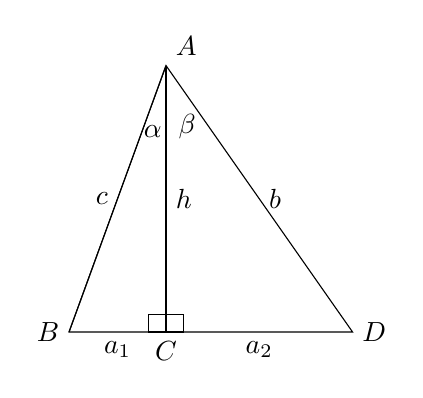
\begin{tikzpicture}[scale=.9]
\coordinate (B) at (0,0);
\node[left] at (B) {$B$};
\coordinate (D) at (4,0);
\node[right] at (D) {$D$};
\draw (B) -- +(70:4) coordinate (A);
\node[above right] at (A) {$A$};
\draw (A) -- node[left] {$c$} (B) -- (D) -- node[right] {$b$} cycle;

\draw (A) -- node[right] {$h$} (A|-B) coordinate (C);
\node[below] at (C) {$C$};
\node[below left,xshift=2pt,yshift=-18pt] at (A) {$\alpha$};
\node[below right,xshift=1pt,yshift=-14pt] at (A) {$\beta$};
\draw[rotate=90] (C) rectangle +(7pt,7pt);
\draw (C) rectangle +(7pt,7pt);
\path (B) -- node[below] {$a_1$} (C) -- node[below] {$a_2$} (D);
\end{tikzpicture}
\end{center}
\caption{Computation of the area of a triangle in two ways}\label{f.sin-sum2}
\end{figure}

\enlargethispage{\baselineskip}

The second proof uses the following theorem:
\begin{theorem}
In a circle of \emph{diameter} $1$ the length of a chord that subtends an inscribed angle is equal to the sine of the angle (Fig.~\ref{f.chord-angle}).
\end{theorem}

\begin{figure}[b]
\begin{center}
\begin{tikzpicture}[scale=.7]

\coordinate (A) at (0,0);
\coordinate (C) at (3,4);
\coordinate (O) at ($(A)!.5!(C)$);
\vertex{O};
\node[left] at (O) {$O$};
\draw (A) -- (C);
\node[draw,circle through=(A),name path=circle] at (O) {};
\coordinate (B) at ($(O)+(10:2.5)$);
\draw (A) -- (B) -- node[left] {$a$} (C);
\draw[rotate=120] (B) rectangle +(8pt,8pt);
\coordinate (D) at ($(O)+(160:2.5)$);
\draw(C) -- (D) -- (B);
\node[above right,xshift=12pt,yshift=12pt] at (A) {$\alpha$};
\node[right,xshift=16pt,yshift=2pt] at (D) {$\alpha$};
\node[below left] at (A) {$A$};
\node[above right] at (C) {$B$};
\node[right] at (B) {$C$};
\node[left] at (D) {$D$};
\end{tikzpicture}
\end{center}
\caption{All inscribed angles subtended by a chord are equal}\label{f.chord-angle}
\end{figure}

\begin{proof}
Let $\overline{AB}$ be a diameter and let $\angle BAC=\alpha$. Let $D$ be any other point on the circle one of whose sides is the chord $\overline{BC}$. Since equal chords subtend equal inscribed angles $\angle BDC=\alpha$. In the right triangle $\triangle ABC$:
\[
\sin \alpha = \frac{\overline{BC}}{\overline{AB}}=\frac{\overline{BC}}{1}=\overline{BC}\,.
\]
\end{proof}

\begin{proof}[2]
This proof is based on the right diagram in Fig.~\ref{f.sin-sum1} reproduced in Fig.~\ref{f.trig-quad-circle}, where the quadrilateral $\overline{ABCD}$ has been inscribed in a circle.\index{Quadrilateral!inscribed in a circle}
By Thm.~\ref{thm.quad-circum} a quadrilateral can be circumscribed\index{Circumscribed circle} by a circle if and only if the sum of each pair of opposite angles is $180^\circ$.
$\angle ADC+\angle ABC=180^\circ$ since both angles are right angles. From Thm.~\ref{thm.interior-angles-of-a-polygon} the sum of the interior angles of a quadrilateral is $360^\circ$, so $\angle DAB+\angle DCB=180^\circ$. 
\begin{figure}[t]
\begin{center}
\begin{tikzpicture}[scale=.8]
\coordinate (A) at (0,0);
\node[left] at (A) {$A$};
\node[right,xshift=6pt,yshift=5pt] at (A) {$\alpha$};
\node[above right,xshift=4pt,yshift=8pt] at (A) {$\beta$};
\coordinate (B) at (3.5,0);
\node[right] at (B) {$B$};
\draw (A) -- +(70:4.5) coordinate (D);
\node[above left] at (D) {$D$};
\path[name path=dc1] (D) -- +(-20:2.5);
\path[name path=bc1] (B) -- +(90:4);
\path[name intersections={of=dc1 and bc1,by={C}}];
\node[above right] at (C) {$C$};
\draw[rotate=90] (B) rectangle +(9pt,9pt);
\draw[rotate=-110] (D) rectangle +(9pt,9pt);
\draw (A) -- (B) -- (C) -- (D) -- cycle;
\draw (A) -- (C);
\draw (D) -- (B);

\coordinate (O) at ($(A)!.5!(C)$);
\node[draw,circle through=(A),name path=circle] at (O) {};
\node[below right,xshift=6pt,yshift=-4pt] at (D) {$\alpha$};
\node[below,xshift=1pt,yshift=-10pt] at (D) {$\gamma$};
\node[below left,xshift=-6pt,yshift=4pt] at (C) {$\delta$};
\node[below,xshift=-4pt,yshift=-6pt] at (C) {$\gamma$};
\node[above left,xshift=-7pt,yshift=4pt] at (B) {$\delta$};
\node[above,xshift=-4pt,yshift=14pt] at (B) {$\beta$};
\end{tikzpicture}
\end{center}
\caption{A quadrilateral circumscribed by a circle}\label{f.trig-quad-circle}
\end{figure}

Let the diameter of the circle be $1$ (otherwise, multiply everything by the length of the diameter). Then the sides of the quadrilateral are:
\[
\overline{BC}=\sin\alpha,\quad \overline{CD}=\sin\beta,\quad \overline{AB}=\sin\gamma,\quad \overline{DA}=\sin\delta\,,
\]
and their diagonals are:
\[
\overline{BD}=\sin(\alpha + \beta),\quad \overline{CA}=\sin (\alpha+\gamma)\,.
\]

By Ptolemy's Theorem\index{Ptolemy's theorem} (Thm.~\ref{thm.ptolemy}) the product of the diagonals of a quadrilateral circumscribed by a circle is equal to the sum of the products of opposite sides of the quadrilateral. Since $\angle ADC$ and $\angle ABC$ are right angles we have:
\[
\renewcommand{\arraystretch}{1.3}
\begin{array}{lcl}
\sin (\alpha+\beta)\sin(\alpha+\gamma)&=&
\sin \alpha \sin\delta + \sin \beta\sin \gamma\\
\sin (\alpha+\beta)\sin(90^\circ)&=&
\sin \alpha \sin(90^\circ-\beta) + \sin \beta\sin (90^\circ-\alpha)\\
\sin (\alpha+\beta)&=&\sin\alpha\cos\beta+\cos\alpha\sin \beta\,.
\end{array}
\]
\end{proof}

%%%%%%%%%%%%%%%%%%%%%%%%%%%%%%%%%%%%%%%%%%%%%%%%%%%%%%%%%%%

\subsection{The Cosine of a Triple Angle}\label{s.cosine}
\index{Trigonometric identities!cosine of a triple angle}
\begin{theorem}\label{thm.triple-angle}
\[
\cos 3\alpha=4\cos^3\alpha -3\cos\alpha\,.
\]
\end{theorem}
\begin{proof}
The proof uses the formulas in Thm.~\ref{thm.sum-of-trig} and the formula $\sin^2\alpha+\cos^2\alpha=1$:
\begin{eqnarray*}
\cos 3\alpha &=& \cos (2\alpha +\alpha)\\
&=& \cos 2\alpha\cos\alpha - \sin 2\alpha\sin\alpha\\
&=& (\cos^2\alpha -\sin^2\alpha)\cos\alpha - (2\sin\alpha\cos\alpha)\sin\alpha\\
&=&\cos^3\alpha - \cos\alpha\sin^2\alpha -2\sin^2\alpha\cos\alpha)\\
&=&\cos^3\alpha - \cos\alpha +\cos^3\alpha -2\cos\alpha+2\cos^3\alpha\\
&=&4\cos^3\alpha -3\cos\alpha\,.
\end{eqnarray*}
\end{proof}

%%%%%%%%%%%%%%%%%%%%%%%%%%%%%%%%%%%%%%%%%%%%%%%%%%%%%%%%%%%

\subsection{The Sine and Cosine of a Half-Angle}\label{s.sine-cosine-half}
\index{Trigonometric identities!sine and cosine of a half-angle}
\begin{theorem}\label{thm.sine-cosine-half}
If $\alpha$ is an angle in a \emph{triangle} then:\footnote{The general formula is more complex  because the square roots can be either positive or negative depending on the quadrant in which $\alpha/2$ is located. For a triangle $0\!<\!\alpha\!<\!180^\circ$, so $0\!<\!\alpha/2\!<\!90^\circ$ is in the first quadrant and both the sine and the cosine are positive.}
\begin{eqnarray*}
\cos \left(\frac{\alpha}{2}\right)&=&\sqrt{\frac{1+\cos\alpha}{2}}\\
\sin\left(\frac{\alpha}{2}\right)&=&\sqrt{\frac{1-\cos\alpha}{2}}\,.
\end{eqnarray*}
\end{theorem}

\begin{proof}
The proof uses the formulas Thm.~\ref{thm.sum-of-trig} and the formula $\sin^2\alpha+\cos^2\alpha=1$:
\begin{eqnarray*}
\cos \alpha&=&\cos 2\left(\frac{\alpha}{2}\right)=\cos \left(\frac{\alpha}{2}\right)\cos\left(\frac{\alpha}{2}\right)-\sin \left(\frac{\alpha}{2}\right)\sin\left(\frac{\alpha}{2}\right)\\
&=&2\cos^2 \left(\frac{\alpha}{2}\right)-1\\
\cos \left(\frac{\alpha}{2}\right)&=&\sqrt{\frac{1+\cos\alpha}{2}}\\
\sin^2\left(\frac{\alpha}{2}\right)&=& 1-\cos^2\left(\frac{\alpha}{2}\right)=1-\frac{1+\cos\alpha}{2}\\
\sin \left(\frac{\alpha}{2}\right)&=&\sqrt{\frac{1-\cos\alpha}{2}}\,.
\end{eqnarray*}
\end{proof}

%%%%%%%%%%%%%%%%%%%%%%%%%%%%%%%%%%%%%%%%%%%%%%%%%%%%%%%%%%%

\subsection{The Law of Cosines}

\begin{theorem}[Law of cosines]
In  a triangle $\triangle ABC$ with sides $a,b,c$ (Fig.~\ref{f.law-cosines2}):\label{thm.law-of-cosines}\index{Law of cosines}
\[
c^2=a^2+b^2-2ab\cos \angle ACB\,.
\]
\end{theorem}

\begin{proof}[1]
Drop an an altitude from $C$ to $\overline{AB}$ and use the definition of cosine and Pythagoras's Theorem:
\begin{subeqnarray}
c&=& x+(c-x)=a\cos \beta + b\cos \alpha\\
c^2&=&ac\cos \beta + bc\cos \alpha\,.\slabel{eq.lc1}
\end{subeqnarray}
Similarly, drop altitudes from $A$ to $\overline{BC}$ and from $B$ to $\overline{AC}$ to obtain:
\begin{subeqnarray}
a^2&=&ca\cos \beta + ba\cos \gamma\slabel{eq.lc2}\\
b^2&=&cb\cos \alpha + ab\cos \gamma\,.\slabel{eq.lc3}
\end{subeqnarray}

Adding Eqs.~\ref{eq.lc2} and \ref{eq.lc3} and subtracting Eq.~\ref{eq.lc1} gives:
\begin{eqnarray*}
a^2+b^2-c^2&=&ca\cos \beta + ba\cos \gamma\\
&&\;\; +\,cb\cos \alpha + ab\cos \gamma \\
&&\;\; -\,ac\cos \beta - bc\cos \alpha\\
&=&2ab\cos \gamma\\
c^2&=&a^2+b^2-2ab\cos \gamma\,.
\end{eqnarray*}
\end{proof}

\begin{figure}[b]
\begin{center}
\begin{tikzpicture}[scale=.65]
  \coordinate[label = left:$A$] (A) at (0,0);
  \coordinate[label = right:$B$] (B) at (6,0);
  \draw (A) -- (40:5) coordinate (C) node[above] {$C$};
  \draw (A) -- (B) -- node[right] {$a$} (C) -- node[left,yshift=4pt,xshift=-2pt] {$b$} cycle;
\node[below,xshift=-4pt,yshift=-6pt] at (C) {$\gamma$};
\node[above right,xshift=8pt] at (A) {$\alpha$};
\node[above left,xshift=-8pt] at (B) {$\beta$};
\coordinate (D) at (A-|C);
\draw (C) -- (D);  
\draw (D) rectangle +(10pt,10pt);
\draw[<->] (0,-.5) -- node[fill=white] {$c$} (6,-0.5);
\draw[<->] (0,-1) -- node[fill=white] {$c-x$} ($(D)+(0,-1)$);
\draw[<->] ($(D)+(0,-1)$) -- node[fill=white] {$x$} (6,-1);
\end{tikzpicture}
\caption{Proof 1 of the Law of Cosines}\label{f.law-cosines2}
\end{center}
\end{figure}

\newpage


\begin{proof}[2]
The second proof uses Ptolemy's theorem (Thm.~\ref{thm.ptolemy}).\footnote{Section~\ref{a.ptolemy} uses the Law of Cosines to prove Ptolemy's theorem! The first proof of the Law of Cosines avoids this circular reasoning. Furthermore, there are proofs of Ptolemy's theorem that do not use the Law of Cosines.}

The triangle $\triangle ABC$ can be circumscribed by a circle. 
Construct another triangle $\triangle ABC'$ congruent with $\triangle ABC$ and inscribed within the same circle (Fig.~\ref{f.law-cosines3}). This can be done by constructing an angle from $\overline{AB}$ equal to $\angle CAB$ which intersects the circle at $C'$ and then constructing the line $\overline{C'A}$.
Since angles that are subtended by the same chord are equal $\angle AC'B =\angle BCA$, so also $\angle CBA=\angle C'AB$ and thus $\triangle ABC'\cong\triangle BAC$ by angle-side-angle with the common side $\overline{AB}$.

Drop perpendiculars from $C$ to $D$ and from $C'$ to $D'$ on $\overline{AB}$ so that $x=a\cos \beta$. By Ptolemy's theorem for the quadrilateral $\overline{ABCC'}$:
\begin{eqnarray*}
b^2&=&a^2+c(c-2x)\\
&=& a^2 + c(c-2a\cos\beta)\\
&=&a^2+c^2-2ac\cos\beta\,.
\end{eqnarray*}
\end{proof}

\begin{figure}[b]
\begin{center}
\begin{tikzpicture}[scale=.8]
\coordinate (origin) at (0,0);
\coordinate (A) at (-3,-1.5);
\coordinate (B) at (3,-1.5);
\node[draw,circle through=(A),name path=circle] at (origin) {};
\node[left] at (A) {$A$};
\node[right] at (B) {$B$};
\path[name path=b1] (A) -- +(40:7cm);
\path[name path=b2] (B) -- +(140:7cm);
\path [name intersections={of=circle and b1,by={C}}];
\node[above] at (C) {$C$};
\path [name intersections={of=circle and b2,by={Cp}}];
\node[above] at (Cp) {$C'$};
\draw (A) -- node[below] {$c$} (B) -- node[right] {$a$} (C) -- node[left,yshift=4pt,xshift=-2pt] {$b$} cycle;
\draw (A) -- (B) -- node[right,yshift=4pt,xshift=2pt] {$b$}(Cp) -- node[left] {$a$} cycle;
\draw (C) -- node[above] {$c-2x$} (Cp);
\coordinate (D) at (C|-B);
\coordinate (Dp) at (Cp|-B);
\draw (C) -- (D);
\draw[rotate=90] (D) rectangle +(8pt,8pt);
\draw (Cp) -- (Dp);
\draw (Dp) rectangle +(8pt,8pt);
\draw[<->] ($(A)+(0,-.8)$) -- node[fill=white] {$x$} ($(Dp)+(0,-.8)$);
\draw[<->] ($(Dp)+(0,-.8)$) -- node[fill=white] {$c-2x$} ($(D)+(0,-.8)$);
\draw[<->] ($(D)+(0,-.8)$) -- node[fill=white] {$x$} ($(B)+(0,-.8)$);
\node[below] at (D) {$D$};
\node[below] at (Dp) {$D'$};
\node[above right,xshift=8pt,yshift=6pt] at (B) {$\beta$};
\draw ($(B)+(-.8,0)$) arc (180:104:.8);
\draw[->] ($(B)+(.4,.5)$) -- +(190:1.12);

\node[above left,xshift=-8pt,yshift=6pt] at (A) {$\beta$};
\draw ($(A)+(.8,0)$) arc (0:76:.8);
\draw[->] ($(A)+(-.4,.5)$) -- +(-10:1.12);
\end{tikzpicture}
\end{center}
\caption{Proof 2 of the Law of Cosines}\label{f.law-cosines3}
\end{figure}                       

%%%%%%%%%%%%%%%%%%%%%%%%%%%%%%%%%%%%%%%%%%%%%%%%%%%%%%%%%%%

\newpage

\subsection{The Tangent of the Sum of Two Angles}\label{s.tangent-sum}
\index{Trigonometric identities!tangent of the sum of two angles}

\begin{theorem}\label{thm.tangent-sum}
\[
\tan (\alpha+\beta) =\frac{\tan\alpha+\tan\beta}{1-\tan\alpha\tan\beta}\,.
\]
\end{theorem}

\begin{proof}

\begin{eqnarray*}
\tan (\alpha+\beta) &=& \frac{\sin(\alpha+\beta)}{\cos(\alpha+\beta)}\\
&=&\frac{\sin\alpha\cos\beta+\cos\alpha\sin\beta}{\cos\alpha\cos\beta-\sin\alpha\sin\beta}\\
&=&\frac{\sin\alpha+\cos\alpha\tan\beta}{\cos\alpha-\sin\alpha\tan\beta}\\
&=&\frac{\tan\alpha+\tan\beta}{1-\tan\alpha\tan\beta}\,.
\end{eqnarray*}

\end{proof}

%%%%%%%%%%%%%%%%%%%%%%%%%%%%%%%%%%%%%%%%%%%%%%%%%%%%%%%%%%%

\subsection{The Tangent of a Half-Angle}\label{s.tangent-half}
\index{Trigonometric identities!tangent of a half-angle}
\begin{theorem}\label{thm.tangent-half}
\[
\tan\left(\frac{\alpha}{2}\right) = \frac{-1\pm\sqrt{1+\tan^2\alpha}}{\tan\alpha}\,.
\]
\end{theorem}
\begin{proof}
We derive and solve a quadratic equation in $\displaystyle\tan\left(\displaystyle\frac{\alpha}{2}\right)$:
\begin{displaymath}
\begin{array}{lll}
\tan \alpha&=&\displaystyle\frac{
  \tan\left(\displaystyle\frac{\alpha}{2}\right)+
  \tan\left(\displaystyle\frac{\alpha}{2}\right)
  }{
  1-\tan\left(\displaystyle\frac{\alpha}{2}\right)
    \tan\left(\displaystyle\frac{\alpha}{2}\right)
  }\\
\tan\alpha \tan^2  \left(\displaystyle\frac{\alpha}{2}\right) + 2 \tan \left(\displaystyle\frac{\alpha}{2}\right) -\tan\alpha &=&0\\
\tan\left(\displaystyle\frac{\alpha}{2}\right) &=& \displaystyle\frac{-1\pm\sqrt{1+\tan^2\alpha}}{\tan\alpha}\,.
\end{array}
\end{displaymath}
\end{proof}

%%%%%%%%%%%%%%%%%%%%%%%%%%%%%%%%%%%%%%%%%%%%%%%%%%%%%%%%%%%

\newpage

\subsection{The Product of Three Tangents}\label{s.tangent-three}
\index{Trigonometric identities!product of three tangents}
\begin{theorem}\label{thm.tangent3}
If $\alpha+\beta+\gamma=180^\circ$ then:
\[
\tan\alpha+\tan\beta+\tan\gamma = \tan\alpha\tan\beta\tan\gamma\,.
\]
\end{theorem}

\begin{proof}
\begin{eqnarray*}
\tan\gamma &=& \tan (180^\circ-(\alpha+\beta))\\
&=& -\tan (\alpha+\beta)\\
&=& -\frac{\tan\alpha+\tan\beta}{1-\tan\alpha\tan\beta}\\
\tan\alpha\tan\beta\tan\gamma &=&\tan\alpha+\tan\beta+\tan\gamma\,.
\end{eqnarray*}

\end{proof}

%%%%%%%%%%%%%%%%%%%%%%%%%%%%%%%%%%%%%%%%%%%%%%%%%%%%%%%%%%%


\begin{figure}[b]
\begin{center}
\begin{tikzpicture}[scale=.7]
\coordinate (o1) at (0,0);
\coordinate (a1) at (1.8,0);
\node[draw, name path = circle] at (o1)
    [circle through = (a1)] {};
\foreach \node/\angle in {a2/120,a3/240} {
  \coordinate (\node) at (\angle:1.8);
}
\draw (a1) -- (a2) -- (a3) -- cycle;
\begin{scope}[xshift=5cm]
\coordinate (o2) at (0,0);
\coordinate (b1) at (1.8,0);
\node[draw, name path = circle] at (o2)
    [circle through = (b1)] {};
\foreach \node/\angle in
  {b2/45,b3/90,b4/135,b5/180,b6/-135,b7/-90,b8/-45} {
  \coordinate (\node) at (\angle:1.8);
}
\draw (b1) -- (b2) -- (b3) -- (b4) -- (b5) -- (b6) -- (b7) -- (b8) -- cycle;
\end{scope}
\begin{scope}[xshift=10cm]
\coordinate (o3) at (0,0);
\coordinate (c1) at (1.8,0);
\node[draw, name path = circle] at (o3)
    [circle through = (c1)] {};
\foreach \node/\angle in
  {c2/22.5,c3/45,c4/67.5,c5/90,c6/112.5,c7/135,
   c8/157.5,c9/180,c16/-22.5,c15/-45,c14/-67.5,
   c13/-90,c12/-112.5,c11/-135,c10/-157.5} {
  \coordinate (\node) at (\angle:1.8);
}
\draw (c1) -- (c2) -- (c3) -- (c4) -- (c5) -- (c6) --
  (c7) -- (c8) -- (c9) -- (c10) -- (c11) -- (c12) -- (c13) --
  (c14) -- (c15) -- (c16) -- cycle;
\end{scope}
\end{tikzpicture}
\caption{Regular polygons with $3$, $8$ and $16$ sides inscribed within a circle}\label{fig.regular-polygons}
\end{center}
\end{figure}

\subsection{The Limit of $\sin\alpha/\alpha$}\label{s.sin-over-x}
\index{Trigonometric identities!limit@limit of $\sin \alpha/\alpha$}

\begin{theorem}\label{thm.limit-sine-over}
\[
\lim_{\alpha\rightarrow 0}\frac{\sin\alpha}{\alpha}=1\,.
\]
\end{theorem}

\begin{proof}
By examining  regular polygons inscribed within a circle (Fig.~\ref{fig.regular-polygons}), we see that the more sides that a polygon has, the closer its perimeter is to the circumference of the circle. The circumference of the circle divided by the number of sides is the length of an arc with the same endpoints as the corresponding side, since in a regular polygon all sides have the same length. Since the ratio of the circumference of the circle to the perimeter of an inscribed polygon approaches $1$ as the number of sides increases, so does the ratio of the length of an arc to the corresponding chord. This is demonstrated by the following numerical examples:

\enlargethispage{\baselineskip}
\vspace{-1ex}

\[
\begin{array}{r@{\hspace{10pt}}r@{\hspace{10pt}}r@{\hspace{10pt}}r}
\hline
\textrm{Angle} & \textrm{Arc length} & \textrm{Chord length} & \textrm{Ratio}\\\svhline
80 & 1.396 & 1.286  & 1.090\\
60 & 1.047 & 1.000  & 1.047\\
40 & 0.698 & 0.684 & 1.006\\
5  & 0.087 & 0.087 &1.000 \\\hline
\end{array}
\]

Since $a=b=1$ the length of the chord $c$ subtending $\alpha$ can be computed from the Law of Cosines \index{Law of cosines} (Fig.~\ref{fig.length-of-a-chord}):
\begin{figure}[t]
\begin{center}
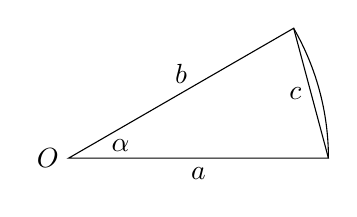
\begin{tikzpicture}[scale=1.1]
  \coordinate  (A) at (3,0);
  \coordinate[label = left:$O$] (O) at (0,0);
  \vertex{O};
  \draw (A) arc(0:30:3) coordinate (B);
  \draw (A) -- node[below] {$a$} (O) -- node[above] {$b$} (B) -- node[left] {$c$} cycle;
  \node[above right,xshift=12pt,yshift=-1pt] at (O) {$\alpha$};
\end{tikzpicture}
\caption{The length of a chord corresponding to an arc of size $\alpha$}\label{fig.length-of-a-chord}
\end{center}
\end{figure}
\begin{eqnarray*}
c^2&=&a^2+b^2-2ab\cos \alpha\\
c&=&\sqrt{2-2\cos \alpha}\\
\lim_{\alpha\rightarrow 0} c&=& \sqrt{2-2\cdot 1}=0\,.
\end{eqnarray*}
Referring to Fig.~\ref{fig.ratio-of-sine-to-x}:
\[
\lim_{\alpha \rightarrow 0} \frac{\sin \alpha}{\alpha} = \lim_{\alpha \rightarrow 0} \frac{2\sin \alpha}{2\alpha}\,.
\]
This is the ratio of the length of chord $\overline{PQ}$ to the length of arc $\widehat{PQ}$.
But we have seen that this ratio converges to $1$ as the subtended angle $2\alpha$ tends to $0$, so:
\[
\lim_{\alpha \rightarrow 0} \frac{\sin \alpha}{\alpha} = 1\,.
\]
\end{proof}
\index{Trigonometric identities|)}

\begin{figure}[h]
\begin{center}
\begin{tikzpicture}[scale=.9]
  \draw[thin] (-2,0) -- (2,0);
  \draw[thin] (0,-2) -- (0,2);
  \coordinate[label = above left:$A$]  (A) at (-2,0);
  \coordinate[label = above right:$B$] (B) at (2,0);
  \coordinate[label = above left:$O$] (O) at (0,0);
\vertex{O};
  \node[above right,xshift=6pt] at (O) {$\alpha$} 
    node[below right,xshift=6pt] {$\alpha$};
  \coordinate (P) at (40:2);
  \node[above right] at (P) {$P$};
  \coordinate (Q) at (-40:2);
  \node[draw, name path = circle] at (O)
    [circle through = (A)] {};
  \draw (B)
    arc[start angle=0,end angle=40,radius=2cm];
  \draw (B)
    arc[start angle=0,end angle=-40,radius=2cm];
  \node at (2.1,.8) {$\alpha$};
  \node at (2.1,-.8) {$\alpha$};
  \draw[<->] (P) -- node[fill=white,xshift=-4pt] {$\sin \alpha$}
    (P |- O) coordinate (D);
  \draw[<->] (D) -- node[fill=white,xshift=-4pt] {$\sin \alpha$} (Q);
  \node[below right] at (Q) {$Q$};
  \draw (Q) -- node[below] {$1$} (O) -- node[above] {$1$} (P);
\end{tikzpicture}
\caption{Ratio of $\sin x$ to $x$}\label{fig.ratio-of-sine-to-x}
\end{center}
\end{figure}

%%%%%%%%%%%%%%%%%%%%%%%%%%%%%%%%%%%%%%%%%%%%%%%%%%%%%%%%%%%

\newpage

\section{The Angle Bisector Theorems}\label{a.bisector}
\index{Triangle!angle bisector theorem}

\begin{theorem}\label{thm.angle-bisector}
In $\triangle ABC$ let the angle bisector of $\angle BAC$ intersect $\overline{BC}$ at $D$ (Fig.~\ref{f.angle-bisector}). Then:
\[
\frac {\overline{BD}}{\overline{CD}}=\frac {\overline{AB}}{\overline{AC}}\,.
\]
\end{theorem}

\begin{figure}[b]
\begin{center}
\begin{tikzpicture}[scale=.8]
% Draw base and path two lines at known angles
\draw (0,0) coordinate (b) node[left] {$B$} -- (8,0) coordinate (c) node[right] {$C$};
\path[name path=ba] (b) -- +(50:4.5);
\path[name path=ca] (c) -- +(150:7);
% Get their intersection and draw lines between vertices
\path[name intersections={of=ba and ca,by=a}];
\node[above] at (a) {$A$};
\draw (a) -- (c) -- (b) -- (a);
\path[name path=bc] (b) -- (c);
\path[name path=bisector] (a) -- +(-80:4);
\path[name intersections={of= bc and bisector,by=d}];
\node[below] at (d) {$D$};
\draw (a) -- (d);
\node[below left,xshift=2pt,yshift=-8pt] at (a) {$\alpha$};
\node[below right,xshift=2pt,yshift=-8pt] at (a) {$\alpha$};
\draw (a) -- node[left] {$h$} (a |- b);
\draw (a|-b) rectangle +(7pt,7pt);
\end{tikzpicture}
\end{center}
\caption{The internal angle bisector theorem}\label{f.angle-bisector}
\end{figure}
\begin{proof}
We prove the theorem by computing the areas of two triangles using both the base and height (Eq.~\ref{eq.area-from-base}), and the base, angle and side (Eq.~\ref{eq.area-from-sine}):
\begin{eqnarray*}
\triangle ABD&=&\frac{1}{2}\overline{BD}h=\frac{1}{2}\overline{AB}\,\overline{AD}\sin \alpha\\
\frac{\overline{BD}}{\overline{AB}}&=&\frac{\overline{AD}\sin \alpha}{h}\\
\triangle ACD&=&\frac{1}{2}\overline{CD}h=\frac{1}{2}\overline{AC}\,\overline{AD}\sin \alpha\\
\frac{\overline{CD}}{\overline{AC}}&=&\frac{\overline{AD}\sin \alpha}{h}\\
\frac{\overline{BD}}{\overline{CD}}&=&\frac{\overline{AB}}{\overline{AC}}\,.
\end{eqnarray*}
\end{proof}

There is also an angle bisector theorem for the \emph{external bisector}:
\index{Triangle!angle bisector theorem}
\begin{theorem}\label{thm.external-angle-bisector}
In $\triangle ABC$ let $\overline{AE}$ be the bisector of the angle supplementary to the angle $\triangle BAC$ (Fig.~\ref{f.angle-bisector-external}) and let the bisector intersect $\overline{BC}$ at $E$ (Fig.~\ref{f.angle-bisector}). Then:
\[
\frac {\overline{BE}}{\overline{CE}}=\frac {\overline{AB}}{\overline{AC}}\,.
\]
\end{theorem}

\begin{figure}[t]
\begin{center}
\begin{tikzpicture}[scale=1]
% Draw base and path two lines at known angles
\draw (0,0) coordinate (b) node[below] {$B$} -- (6,0) coordinate (c) node[right] {$C$};
\path[name path=ba] (b) -- +(70:2.5);
\draw[name path=ca] (c) -- +(160:7);
% Get their intersection and draw lines between vertices
\path[name intersections={of=ba and ca,by=a}];
\node[above] at (a) {$A$};
\draw (a) -- (c) -- (b) -- (a);
\path[name path=bc] (b) -- (c);
\node[left,xshift=-10pt,yshift=-2pt] at (a) {$\alpha$};
\node[below,xshift=-12pt,yshift=-8pt] at (a) {$\alpha$};
\path[name path=ext-bisector] (a) -- +(-155:4.7);
\draw[name path=ext-bc] (c) -- ($(c)!1.6!(b)$);
\path[name intersections={of=ext-bc and ext-bisector,by=e}];
\draw (a) -- (e) node[below] {$E$};
\coordinate (d) at (a |- b);
\draw (a) -- node[right] {$h$} (d);
\draw (d) rectangle +(6pt,6pt);
\end{tikzpicture}
\end{center}
\caption{The external angle bisector theorem}\label{f.angle-bisector-external}
\end{figure}

\newpage

\begin{proof} Since $\overline{AC}$ is a straight line $\angle EAC=180^\circ-\alpha$.
\begin{eqnarray*}
\triangle ABE&=&\frac{1}{2}\overline{BE}h=\frac{1}{2}\overline{AE}\,\overline{AB}\sin \alpha\\
\triangle ACE&=&\frac{1}{2}\overline{CE}h=\frac{1}{2}\overline{AE}\,\overline{AC}\sin (180^\circ-\alpha)=\frac{1}{2}\overline{AE}\,\overline{AC}\sin \alpha\\
\frac{\overline{BE}}{\overline{AB}}&=&\frac{\overline{AE}\sin \alpha}{h}=\frac{\overline{CE}}{\overline{AC}}\\
\frac{\overline{BE}}{\overline{CE}}&=&\frac{\overline{AB}}{\overline{AC}}\,.
\end{eqnarray*}
\end{proof}

%%%%%%%%%%%%%%%%%%%%%%%%%%%%%%%%%%%%%%%%%%%%%%%%%%%%%%%%%%%

\section{Ptolemy's Theorem}\label{a.ptolemy}
\index{Ptolemy's theorem}

%%%%%%%%%%%%%%%%%%%%%%%%%%%%%%%%%%%%%%%%%%%%%%%%%%%%%%%%%%%

\subsection{A Trapezoid Circumscribed by a Circle}\label{s.circumscribed}

Before giving the proof of Ptolemy's theorem we prove theorems on quadrilaterals and trapezoids.

\begin{theorem}\label{thm.quad-circum}
A quadrilateral can be circumscribed by a circle if and only if the opposite angles are supplementary (sum to $180^\circ$).
\end{theorem}\index{Circumscribed circle}

Geometry textbooks give the simple proof of the forward direction, but it is hard to find a proof of the converse so both proofs are given here.

\begin{proof}[Forward direction]
An inscribed angle is equal to half the arc that subtends it so $\angle DAB$ is half of the arc $\widehat{DCB}$ and $\angle DCB$ is half of the arc $\widehat{DAB}$ (Fig.~\ref{f.trap-1}). The two arcs form the entire circumference of the circle so their sum is $360^\circ$. Therefore, $\angle DAB + \angle DCB = \frac{1}{2} \cdot 360^\circ =  180^\circ$, and similarly $\angle ADC + \angle ABC = 180^\circ$.

\end{proof}

\begin{figure}[ht]
\subfigures
\leftfigure[c]{
\begin{tikzpicture}[scale=.55]
\coordinate (origin) at (0,0);
\coordinate (A) at (1,3);
\node[draw,circle through=(A),name path=circle] at (origin) {};
\node[above right] at (A) {$A$};
\path[name path=b] (A) -- (-50:4.5cm);
\path[name path=c] (A) -- (-120:4.5cm);
\path[name path=d] (A) -- (150:4.5cm);
\path [name intersections={of=circle and b,by={b1,B}}];
\node[right] at (B) {$B$};
\path [name intersections={of=circle and c,by={c1,C}}];
\node[below left] at (C) {$C$};
\path [name intersections={of=circle and d,by={d1,D}}];
\node[above left] at (D) {$D$};
\draw (A) -- (B) -- (C) -- (D) -- cycle;
\end{tikzpicture}
}
\rightfigure[c]{
\begin{tikzpicture}[scale=.55]
\coordinate (origin) at (0,0);
\coordinate (A) at (1,3);
\node[draw,circle through=(A),name path=circle] at (origin) {};
\node[above right] at (A) {$A$};
\path[name path=b] (A) -- (-50:4cm);
\path[name path=c] (A) -- (-120:4cm);
\path[name path=d] (A) -- (150:4cm);
\path [name intersections={of=circle and b,by={b1,B}}];
\node[right] at (B) {$B$};
\path [name intersections={of=circle and c,by={c1,C}}];
\node[below left] at (C) {$C$};
\path [name intersections={of=circle and d,by={d2,D}}];
\node[above left] at (D) {$D$};
\coordinate (Cp) at ($(C)!.2!(D)$);
\draw (A) -- (B) -- (Cp) -- (D) -- cycle;
\node[left,xshift=1pt,yshift=2pt] at (Cp) {$C'$};
\draw (D) -- (B) -- (C) -- (Cp);
\end{tikzpicture}
}
\leftcaption{A quadrilateral circumscribed by a circle}\label{f.trap-1}
\rightcaption{The fourth vertex must be on the circumference}\label{f.trap-2}
\end{figure}

\newpage

\begin{proof}[Converse direction]
Any triangle can be circumscribed by a circle. Circumscribe $\triangle DAB$ by a circle and suppose that $C'$ is a point such that $\angle DAB + \angle DC'B = 180^\circ$, but $C'$ is \emph{not} on the circumference of the circle. Without loss of generality, let $C'$ be within the circle (Fig.~\ref{f.trap-2}).

Construct a ray that extends $\overline{DC'}$ and let $C$ be its intersection with the circle. $\overline{ABCD}$ is circumscribed by a circle so:\index{Circumscribed circle}
\begin{eqnarray*}
\angle DAB + \angle DCB &=&  180^\circ = \angle DAB + \angle DC'B\\
\angle DCB &=& \angle DC'B\,,
\end{eqnarray*}
which is impossible if $C$ is on the circle and $C'$ is inside the circle.
\end{proof}

\begin{theorem}\label{thm.isoceles-trapezoid}
The opposite angles of an isosceles trapezoid  are supplementary.
\end{theorem}\index{Trapezoid, isoceles}\index{Circumscribed circle!trapezoid@around a trapezoid}
\begin{proof}
Construct the line $\overline{AB'}$ parallel to $\overline{CD}$ (Fig.~\ref{f.trap-3}). $\overline{AB'CD}$ is a parallelogram and $\triangle ABB'$ is an isosceles triangle, so $\angle C= \angle ABB' = \angle AB'B = \angle B$. Similarly, $\angle A = \angle D$. Since the sum of the internal angles of any quadrilateral is equal to $360^\circ$:
\begin{eqnarray*}
\angle A + \angle B + \angle C + \angle D &=& 360^\circ\\
2\angle A + 2 \angle C &=& 360^\circ\\
\angle A +  \angle C &=& 180^\circ\,,
\end{eqnarray*}
and similarly $\angle B +  \angle D = 180^\circ$.
\end{proof}

\begin{theorem}
An isoceles trapezoid can be be circumscribed by a circle.
\end{theorem}
The proof is immediate by Thms.~\ref{thm.quad-circum}, \ref{thm.isoceles-trapezoid}.

\begin{figure}[t]
\begin{center}
\begin{tikzpicture}[scale=.65]
\clip (-4.5,-2) rectangle (4.5,2.8);
\coordinate (origin) at (0,0);
\coordinate (A) at (2.5,1.8);
\node[circle through=(A),name path=circle] at (origin) {};
\node[above right] at (A) {$A$};
\path[name path=b] (A) -- ++(-80:4cm);
\path[name path=d] (A) -- ++(180:6cm);
\path [name intersections={of=circle and b,by={b1,B}}];
\node[below right] at (B) {$B$};
\path [name intersections={of=circle and d,by={d1,D}}];
\node[above left] at (D) {$D$};
\path[name path=c] (D) -- ++(-100:4cm);
\path [name intersections={of=circle and c,by={c1,C}}];
\node[below left] at (C) {$C$};
\draw (A) -- node[right] {$x$} (B);
\draw[name path=bc] (B) -- node[below] {$y$} (C);
\draw (C) -- node[left] {$x$} (D) -- node[above] {$y$} (A);
\path[name path=para] (A) -- ++(-100:4cm);
\path [name intersections={of=para and bc,by={Bp}}];
\node[below left] at (Bp) {$B'$};
\draw (A) -- node[left,xshift=-2pt] {$x$} (Bp);
\end{tikzpicture}
\end{center}
\caption{An isoceles trapezoid}\label{f.trap-3}
\end{figure}

%%%%%%%%%%%%%%%%%%%%%%%%%%%%%%%%%%%%%%%%%%%%%%%%%%%%%%%%%%%
\subsection{Proof of Ptolemy's Theorem}

\begin{theorem}[Ptolemy]Given a quadrilateral circumscribed by a circle, the following formula relates the lengths of the diagonals and the lengths of the sides (Fig.~\ref{f.trig-ptolemy}).\label{thm.ptolemy}\index{Circumscribed circle}
\[
ef = ac + bd\,.
\]
\end{theorem}

\begin{figure}[b]
\begin{center}
\begin{tikzpicture}[scale=.5]
\coordinate (origin) at (0,0);
\coordinate (A) at (1,3);
\node[draw,circle through=(A),name path=circle] at (origin) {};
\node[above right] at (A) {$A$};
\path[name path=b] (A) -- (-50:4cm);
\path[name path=c] (A) -- (-120:4cm);
\path[name path=d] (A) -- (150:4cm);
\path [name intersections={of=circle and b,by={b1,B}}];
\node[right] at (B) {$B$};
\path [name intersections={of=circle and c,by={C,c2}}];
\node[below left] at (C) {$C$};
\path [name intersections={of=circle and d,by={D,d2}}];
\node[above left] at (D) {$D$};
\draw (A) -- node[right] {$a$} (B) -- node[below,yshift=-10pt] {$b$} (C) -- node[left] {$c$} (D) -- node[above,xshift=2pt,yshift=8pt] {$d$}  cycle;
\draw (A) -- node[right,near start] {$e$} (C);
\draw (B) -- node[left,near end,yshift=-6pt] {$f$} (D);
\end{tikzpicture}
\end{center}
\caption{Ptolemy's theorem}\label{f.trig-ptolemy}
\end{figure}                       

\begin{proof}
By the Law of Cosines\index{Law of cosines} for the four triangles $\triangle ABC$, $\triangle ADC$, $\triangle DAB$, $\triangle DCB$:
\begin{eqnarray*}
e^2 &=& a^2 + b^2 - 2ab \cos \angle B\\
e^2 &=& c^2 + d^2 - 2cd \cos \angle D\\
f^2 &=& a^2 + d^2 - 2ad \cos \angle A\\
f^2 &=& b^2 + c^2 - 2bc \cos \angle C\,.
\end{eqnarray*}
$\angle C = 180^\circ - \angle A$ and $\angle D = 180^\circ - \angle B$ because they are opposite angles of a quadrilateral circumscribed by a circle, so $\cos \angle D = - \cos \angle B$ and $\cos \angle C = -\cos \angle A$. Eliminate the cosine term from the above equations to obtain:
\begin{eqnarray*}
e^2(cd+ab)&=&abc^2+abd^2+a^2cd+b^2cd\\
e^2 &=& \frac{(ac+bd)(ad+bc)}{(ab+cd)}\\
f^2 &=& \frac{(ab+cd)(ac+bd)}{(ad+bc)}\,.
\end{eqnarray*}
Multiply the two equations and simplify to get Ptolemy's theorem:
\begin{eqnarray*}
e^2\cdot f^2 &=& (ac+bd)^2\\
ef &=& (ac+bd)\,.
\end{eqnarray*}
\end{proof}

%%%%%%%%%%%%%%%%%%%%%%%%%%%%%%%%%%%%%%%%%%%%%%%%%%%%%%%%%%%

\section{Ceva's Theorem}\label{a.ceva}

\index{Ceva's theorem}
\begin{theorem}[Ceva]
Given line segments from the vertices of a triangle to the opposite edges that intersect in a point, the lengths of the segments satisfy (Fig.~\ref{f.ceva1}):\label{thm.ceva}
\[
\frac{\overline{AM}}{\overline{MB}}\cdot\frac{\overline{BQ}}{\overline{QS}}\cdot\frac{\overline{SP}}{\overline{PA}} = 1\,.
\]
\end{theorem}

\begin{figure}[b]
\begin{center}
\begin{tikzpicture}
\path[name path=pq] (-4,0) -- (4,0);
\draw (-2,-2) node[below left] {$A$} coordinate (A) -- (2,-2) node[below right] {$B$} coordinate (B);
\draw[name path=as] (A) -- ++(50:4cm) node[above] {$S$} coordinate (S);
\draw[name path=sb] (S) -- (B);
\path [name intersections={of=pq and as,by={P}}];
\path [name intersections={of=pq and sb,by={Q}}];
\node[above left] at (P) {$P$};
\node[above right] at (Q) {$Q$};
\draw[name path=pb] (P) -- (B);
\draw[name path=qa] (Q) -- (A);
\path [name intersections={of=pb and qa,by={O}}];
\node[right,xshift=2pt] at (O) {$O$};
\coordinate (M) at (0,-2);
\node[below right] at (M) {$M$};
\draw (S) -- (M);
\end{tikzpicture}
\end{center}
\caption{Ceva's theorem}\label{f.ceva1}
\end{figure}

\begin{proof} If the altitudes of two triangles are equal, their areas are proportional to the bases. In both diagrams in Fig.~\ref{f.ceva2}, the altitudes of the gray triangles are equal, so:
\[
\frac{\triangle BQO}{\triangle SQO} = \frac{\overline{BQ}}{\overline{QS}}\;,\quad\quad \frac{\triangle BQA}{\triangle SQA} = \frac{\overline{BQ}}{\overline{QS}}\;.
\]

By subtracting the areas of the indicated triangles, we get the proportion between the gray triangles shown in Fig.~\ref{f.ceva3}:
\[
\frac{\triangle BOA}{\triangle SOA}=\frac{\triangle BQA - \triangle BQO}{\triangle SQA-\triangle SQO} = \frac{\overline{BQ}}{\overline{QS}}\,.
\]

\begin{figure}[t]
\begin{center}
\begin{tikzpicture}
\clip (-2.2,-2.4) rectangle +(10.4,4);
\path[name path=pq] (-4,0) -- (4,0);
\draw (-2,-2) node[below] {$A$} coordinate (A) -- (2,-2) node[below] {$B$} coordinate (B);
\coordinate (M) at (0,-2);
\draw[name path=as] (A) -- ++(50:4cm) node[above] {$S$} coordinate (S);
\draw[name path=sb] (S) -- (B);
\path [name intersections={of=pq and as,by={P}}];
\path [name intersections={of=pq and sb,by={Q}}];
\path[name path=pb] (P) -- (B);
\path[name path=qa] (Q) -- (A);
\path [name intersections={of=pb and qa,by={O}}];
\draw[fill=gray!40] (B) -- (O) -- (Q);
\draw[fill=gray!70] (S) -- (O) -- (Q);
\draw (B) -- (O) -- (A);
\draw (S) -- (O) -- (A);
\draw (A) -- (B) -- (S) -- cycle;
\draw (S) -- (O);
\draw (B) -- (O);
\node[above right] at (Q) {$Q$};
\node[above left] at (O) {$O$};
\path[name path=al1] (O) -- ($(Q)!(O)!(B)$);
\path [name intersections={of=al1 and sb,by={A1}}];
\draw (O) -- (A1);
\draw[rotate=-156] (A1) rectangle +(7pt,7pt);
\begin{scope}[xshift=6cm]
\path[name path=pq] (-4,0) -- (4,0);
\draw (-2,-2) node[below] {$A$} coordinate (A) -- (2,-2) node[below] {$B$} coordinate (B);
\coordinate (M) at (0,-2);
\draw[name path=as] (A) -- ++(50:4cm) node[above] {$S$} coordinate (S);
\draw[name path=sb] (S) -- (B);
\path [name intersections={of=pq and as,by={P}}];
\path [name intersections={of=pq and sb,by={Q}}];
\draw[name path=pb] (P) -- (B);
\draw[name path=qa] (Q) -- (A);
\path [name intersections={of=pb and qa,by={O}}];
\draw (B) -- (O) -- (Q);
\draw (A) -- (Q) -- (B);
\draw[fill=gray!40] (B) -- (Q) -- (A);
\draw[fill=gray!70] (S) -- (Q) -- (A);
\draw (A) -- (B) -- (S) -- cycle;
\draw (S) -- (O);
\draw (B) -- (O);
\node[above right] at (Q) {$Q$};
\node[above left] at (O) {$O$};
\path[name path=al2] (A) -- ($(Q)!(A)!(B)$);
\path [name intersections={of=al2 and sb,by={A2}}];
\draw (A) -- (A2);
\draw[rotate=-156] (A2) rectangle +(7pt,7pt);
\end{scope}
\end{tikzpicture}
\end{center}
\caption{Triangles in Ceva's theorem}\label{f.ceva2}
\end{figure}

\begin{figure}[b]
\begin{center}
\begin{tikzpicture}
\path[name path=pq] (-4,0) -- (4,0);
\draw (-2,-2) node[below left] {$A$} coordinate (A) -- (2,-2) node[below right] {$B$} coordinate (B);
\coordinate (M) at (0,-2);
\draw[name path=as] (A) -- ++(50:4cm) node[above] {$S$} coordinate (S);
\draw[name path=sb] (S) -- (B);
\path [name intersections={of=pq and as,by={P}}];
\path [name intersections={of=pq and sb,by={Q}}];
\path[name path=pb] (P) -- (B);
\draw[thick,name path=qa] (Q) -- (A);
\path [name intersections={of=pb and qa,by={O}}];
\draw[fill=gray!50] (B) -- (O) -- (A);
\draw[fill=gray!70] (S) -- (O) -- (A);
\draw (B) -- (O) -- (A);
\draw (S) -- (O) -- (A);
\draw (A) -- (B) -- (S) -- cycle;
\draw (S) -- (O);
\draw (B) -- (O);
\node[above right] at (Q) {$Q$};
\node[right,xshift=2pt] at (O) {$O$};
\end{tikzpicture}
\end{center}
\caption{Subtracting areas in Ceva's theorem}\label{f.ceva3}
\end{figure}

This might look strange at first so we explain it using a simpler notation:
\begin{eqnarray*}
 \frac{c}{d} &=&\frac{a}{b}\\
 \frac{e}{f} &=&\frac{a}{b}\\
c-e &=& \frac{ad}{b} - \frac{af}{b}=\frac{a}{b}(d-f)\\
\frac{c-e}{d-f} &=& \frac{a}{b}\,.
\end{eqnarray*}

\newpage

Similarly, we can prove:
\begin{eqnarray*}
\frac{\overline{AM}}{\overline{MB}} &=& \frac{\triangle AOS}{\triangle BOS}\\
\frac{\overline{SP}}{\overline{PA}} &=&\frac{\triangle SOB}{\triangle AOB}\;,
\end{eqnarray*}
so:
\[
\frac{\overline{AM}}{\overline{MB}}\frac{\overline{BQ}}{\overline{QS}}\frac{\overline{SP}}{\overline{PA}} = \frac{\triangle AOS}{\triangle BOS}\frac{\triangle BOA}{\triangle SOA}\frac{\triangle SOB}{\triangle AOB}=1\,,
\]
since the order of the vertices in a triangle makes no difference.
\end{proof}

\begin{figure}[b]
\begin{center}
\begin{tikzpicture}[scale=.6]
\clip (-.8,-.4) rectangle +(11.2,6.5);
\coordinate (D) at (0,0) node[left] {$D$};
\draw (D) -- ++(60:6) coordinate (C) node[left] {$C$};
\coordinate (A) at (60:3);
\node[left] at (A) {$A$};
\draw (A) -- ++(3,0) coordinate (B) -- (C);
\node[below right] at (B) {$B$};
\path[name path=DQ] (D) -- ($(D)!1.7!(B)$);
\path[name path=AP] (A) -- ($(A)!3!(B)$);
% 3*(1+\sqrt[3]{2}) = 6.78
\path[name path=CP] (C) circle (6.78cm);
\path[name intersections={of=CP and AP,by={P}}];
\draw[name path=CP] (C) -- (P);
\path[name intersections={of=CP and DQ,by={Q}}];
\node[above] at (Q) {$Q$};
\node[right] at (P) {$P$};
\draw (D) -- (Q);
\draw (B) -- (P);
\path[dashed,name path=CK] (C) -- ($(C)+(6.5,0)$);
\path[name path=DK] (D) -- ($(D)!2!(Q)$);
\path[name intersections={of=DK and CK,by={K}}];
\draw[dashed] (Q) -- (K) node[right] {$K$} -- (C);
\draw[very thick] (Q) -- (D);
\draw[dashed] (C) -- (K) -- (Q);
\draw (B) -- (P) -- (C);
\end{tikzpicture}
\end{center}
\caption{Menelaus's theorem}\label{f.menelaus}
\end{figure}

\section{Menelaus's Theorem}\label{a.menelaus}

\begin{theorem}[Menelaus]\label{thm.menelaus}\index{Menelaus's theorem}
Let $\triangle ABC$ be a triangle and $\overline{DBQ}$ a \emph{transversal line}  that intersects all three of the edges of the triangle or their extensions (Fig.~\ref{f.menelaus}). Then:\footnote{Depending on the configuration of the triangle and the transversal line, the result of the multiplication can be either plus or minus one.}
\begin{align}
\displaystyle\frac{\overline{AB}}{\overline{BP}}\cdot
\displaystyle\frac{\overline{PQ}}{\overline{QC}}\cdot
\displaystyle\frac{\overline{CD}}{\overline{AD}}=1\,.\label{eq.menelaus}
\end{align}
\end{theorem}

\begin{proof}
Draw a line through $C$ parallel to $\overline{AB}$ and extend $\overline{DQ}$ until it intersects the parallel at $K$. From $\triangle ADB \sim \triangle CDK$ it follows that:
\begin{equation*}
\displaystyle\frac{\overline{CD}}{\overline{AD}}=\displaystyle\frac{\overline{CK}}{\overline{AB}}\,.
\end{equation*}
From $\triangle  BQP\sim \triangle KQC$ it follows that:
\begin{equation*}
\displaystyle\frac{\overline{QC}}{\overline{PQ}}=\displaystyle\frac{\overline{CK}}{\overline{BP}}\,.
\end{equation*}
Eliminating $\overline{CK}$ gives
$\overline{AB}\cdot\overline{CD}\cdot\overline{PQ}=\overline{QC}\cdot\overline{BP}\cdot\overline{AD}$ which can be re-arranged to obtain Thm.~\ref{eq.menelaus}.
\end{proof}

%%%%%%%%%%%%%%%%%%%%%%%%%%%%%%%%%%%%%%%%%%%%%%%%%%%%%%%%%%%

\subsection*{Sources}

The appendix is based primarily on \cite{gelfand}. Ceva's theorem and Menelaus's theorem can be proved from each other \cite{silvester}.
